\footnotetext{Notes from Classical Mechanics by John R. Taylor, ch. 6}

\section{Two example problems}
The calculus of variations can be used to find a function $y(x)$ that minimizes a scalar quantity
that is expressed as an integral $\int_{x_0}^{x_1} f[y(x), y'(x), x] \dx$. Here are two such
problems:

\begin{question*}
  What is the shortest path between two points in a plane?
\end{question*}

\begin{proof}
  Let the points be $(x_0, y_0)$ and $(x_1, y_1)$ and let them be joined by some path $y(x)$ of
  length $S$. Consider a short section of the path of length $\Delta s$ above a section of the
  $x$-axis of length $\Delta x$, and make a linear approximation to the path in this region. The
  length of the hypotenuse is
  \begin{align*}
    \Delta s = \sqrt{(\Delta x)^2 + (y'(x)\Delta x)^2} = \sqrt{1 + y'(x)^2} \Delta x.
  \end{align*}

  Therefore a shortest path is a function $y(x)$ that minimizes
  \begin{align*}
    S[y](x_0, x_1) = \int_{x_0}^{x_1} \sqrt{1 + y'(x)^2}\d x.
  \end{align*}
  with the constraint that the endpoints are fixed at $y(x_0) = y_0$ and $y(x_1) = y_1$.

  \todo{Find the function $y$ that minimizes this integral.}
\end{proof}


\begin{question*}
  In 1662 Fermat proposed that light, when passing from one point to another through a material with
  varying refractive index, takes the path which takes least time\footnote{\todo{In fact, the path
      taken is a stationary point with respect to the action? time? ...not necessarily least}}. What
  is this path?
\end{question*}

\begin{proof}
  Again consider a short section of the path of length $\Delta s$ above a section of the $x$-axis of
  length $\Delta x$. Let $c$ be the speed of light and $n$ be the refractive index in this
  region. This means that the light travels at speed $c/n$, and therefore takes time $(n/c)\Delta s$
  to pass along the hypotenuse. The refractive index $n$ can vary with both $x$ and $y$, therefore a
  least-time path is a function $y(x)$ that minimizes
  \begin{align*}
    T = \int_{x_0}^{x_1} n(x, y(x)) \d s = \int_{x_0}^{x_1} n(x, y(x)) \sqrt{1 + y'(x)^2} \dx,
  \end{align*}
  with the constraint that the endpoints are fixed at $y(x_0) = y_0$ and $y(x_1) = y_1$.

  \todo{Find the function $y$ that minimizes this integral.}
\end{proof}

A naive thought would be to somehow treat $y$ similarly to how a variable is treated when minimizing
a function in in basic calculus, i.e. differentiate the expression with respect to $y$. Recall that
the definition of derivative is
\begin{align*}
  f'(y_0) = \lim_{y_1 \to y_0}\frac{f(y_1) - f(y_0)}{||y_1 - y_0||}.
\end{align*}

\todo{I think this is nonsense and the reason is that multiplication (and therefore division) of
  functions is not defined (they can be treated as vectors, so can be added and scaled, but do not
  have an obviously appropriate multiplication operation). I don't think choosing a norm would
  necessarily be problematic.}

\section{The Euler-Lagrange equations}

\begin{proof}
  Note that in both example problems, the integral to be minimized can be viewed as a scalar-valued
  \emph{functional} $S$ that depends on the \emph{function} $y$:
  \begin{align*}
    S[y](x_0, x_1) = \int_{x_0}^{x_1} f[x, y(x), y'(x)] \dx.
  \end{align*}
  The arguments of the function $f$ that is integrated are \emph{not functions}! They are numeric
  values at a single point in the path: the current $x$ value, the current $y$ value, and current
  slope. We will attempt to stick to a notation wherein a symbol like $y$ is a function, and $y(x)$
  is a result of evaluating the function at input value $x$.

  We'll refer to $S$ as giving the \emph{cost} of traveling along the path $y$, from $(x_0, y_0)$ to
  $(x_1, y_1)$.

  Recall that we seek a least-cost path $y$, subject to the requirement that the endpoints are
  $y(x_0) = y_0$ and $y(x_1) = y_1$. Let $y$ be the least-cost path, and consider an alternative
  path $Y$ whose cost is greater than that of $y$. We can write $Y$ as
  \begin{align*}
    Y = y + \eta,
  \end{align*}
  where we are performing addition on domain-compatible
  functions\footnote{$(f + g)(x) := f(x) + g(x)$}. The difference function $\eta$ must satisfy
  $\eta(x_0) = \eta(x_1) = 0$ in order to restrict the space of functions to those with the same
  endpoints as $y$. Now introduce a parameter $\alpha \in \R$ and redefine $Y$ as\footnote{We are
    adding functions, and we are multiplying a function by a real scalar $\alpha$. The resulting
    function evaluates as $Y(x) = y(x) + \alpha\eta(x).$}
  \begin{align*}
    Y = y + \alpha\eta.
  \end{align*}

  So now we have a family of paths, parameterized by $\alpha$, all satisfying the endpoint
  requirement, and with the least-cost path corresponding to $\alpha=0$. We can reinterpret the cost
  $S$ so that it is a function of $\alpha$:
  \begin{align*}
    S[y](\alpha) &= \int_{x_0}^{x_1} f(x, Y(x), Y'(x)) \dx \\
                 &= \int_{x_0}^{x_1} f\(x, y(x) + \alpha\eta(x), y'(x) + \alpha\eta'(x)\) \dx.
  \end{align*}
  We are trying to find a path $y$ that is a minimum in the cost surface over the function space (or
  a maximum, or saddle point). For such a $y$ it must be the case that\footnote{In traditional
    notation, $\pdv{S}{\alpha}\Big|_{\alpha=0} = 0$.}
  \begin{align*}
    \del_\alpha S[y]\Big|_{\alpha=0} = 0.
  \end{align*}

  So, let's compute $\del_\alpha S[y]$ and use the fact that it must evaluate to zero at $\alpha=0$
  to obtain an equation that $y$ must obey. We'll assume that $f$ satisfies the (mild) conditions
  necessary to ``differentiate under the integral sign'', i.e. that
  \begin{align*}
    \del_\alpha S = \del_\alpha \int_{x_0}^{x_1} f(x, Y(x), Y'(x)) \dx
                 = \int_{x_0}^{x_1} (\del_\alpha f)(x, Y(x), Y'(x)) \dx.
  \end{align*}

  We have
  \begin{align*}
    Y  &= y + \alpha\eta \\
    Y' &= y' + \alpha\eta',
  \end{align*}
  and so from the chain rule we have
  \begin{align*}
    \del_\alpha f &= \del_{Y(x)} f \cdot \del_\alpha Y + \del_{Y'} f \cdot \del_\alpha Y' \\
                 &= \del_{Y} f \cdot \del_\alpha Y + \del_{Y'} f \cdot \del_\alpha Y' \\
  \end{align*}

  \begin{align*}
    \pdv{f(Y, Y', x)}{\alpha} &= \pdv{f}{Y}\pdv{Y}{\alpha} + \pdv{f}{Y'}\pdv{Y'}{\alpha} \\
                              &= \pdv{f}{Y}\eta + \pdv{f}{Y'}\eta'.
  \end{align*}
  Plugging this into the expression for $\pdv*{S}{\alpha}$ and evaluating at $\alpha = 0$ we have
  \begin{align*}
    \int_{x_0}^{x_1} \(\eta\pdv{f}{y} + \eta'\pdv{f}{y'}\) \d x = 0.
  \end{align*}
  (I believe that $Y$ and $Y'$ have now become $y$ and $y'$ because we are evaluating at
  $\alpha=0$.)

  Now, recall integration by parts,
  $\int_a^b u \dv{v}{x} \d x = [uv]_a^b - \int_a^b v\dv{u}{x}\d x$, and apply it to the second term
  inside the integral:
  \begin{align*}
    \int_{x_0}^{x_1} \eta'\pdv{f}{y'} \d x = \Bigg[\eta\pdv{f}{y'}\Bigg]_{x_0}^{x_1} - \int_{x_0}^{x_1} \eta\(\dv{}{x}\pdv{f}{y'}\)\d x.
  \end{align*}
  Because $\eta$ was defined to be the difference between two candidate paths, as noted above we
  have that $\eta(x_0) = \eta(x_1) = 0$. Thus the first term (the ``endpoint term'' or ``boundary
  term'') is zero\footnote{According to Taylor this is common in physics, i.e. that the endpoint
    term is zero and thus integration by parts results in ``switching the prime'' from one factor to
    the other under the integral, and applying a negation.}. So now we have
  \begin{align*}
    \int_{x_0}^{x_1} \eta(x)\(\pdv{f}{y} - \dv{}{x}\pdv{f}{y'}\) \d x = 0.
  \end{align*}
  We now argue that this means that the difference-of-derivatives-function inside the integral is
  zero for all $x$. The reason is basically that this equality is true for \emph{any} $\eta(x)$. So
  suppose the difference-of-derivatives-function were not equal to zero for some $x$. Then we could
  construct an $\eta(x)$ that is non-zero for the same $x$ values that the
  difference-of-derivatives-function is non-zero for, the upshot being that we could construct
  things so that the value of the integral is non-zero; a contradiction. Therefore the
  difference-of-derivatives-function is zero for all $x$, and we have the Euler-Lagrange equations:
  \begin{align*}
    \pdv{f}{y} - \dv{}{x}\pdv{f}{y'} = 0.
  \end{align*}
\end{proof}

This is a system of differential equations which must be satisfied by any path that is stationary
with respect to $f$.

In SICM's functional notation, the Euler-Lagrange system of equations is
\begin{align*}
    (\del_1 f \circ \Gamma[q]) - D(\del_2f \circ \Gamma[q]) = 0,
\end{align*}
where
\begin{itemize}
\item $\Gamma$ is a function mapping time to the tuple of arguments taken by $f$,
  i.e. $\Gamma[q](t) = (t, y(t), y'(t))$,
\item $\del_1$ refers to the partial derivative with respect to position and $\del_2$ is with
  respect to velocity (zero-based indexing of positional arguments).
\end{itemize}

So, any path $q$ for which the action is stationary satisfies the Euler-Lagrange system of
differential equations. And what those equations say is the following:
\begin{enumerate}
\item Recall that $f$ is a function of time, position and velocity values at a single moment in time.
\item Compute the partial derivative function of $f$ with respect to the position argument. Note
  that this is a function of time, position and velocity; its output is a real number (the slope
  of a certain tangent line to the real-valued $f$ surface).
\item Now, form a new function by composing this partial derivative function with $\Gamma[q]$. The
  new function maps time to a real number (the slope). Call this function $A$.
\item Repeat the previous two steps for the velocity argument, instead of the position
  argument. So again, the result is a function mapping time to a real number. But this time, take
  the time derivative of that function. The result is still a function mapping time to a real
  number. Call this function $B$.
\item Now, take a candidate path $q$. If the action is stationary along that path, then at every
  moment $t$ we will find that $A(t) = B(t)$.
\end{enumerate}


\newpage
\subsection{The shortest path between two points on a plane}

\subsubsection{Functional notation}

Let's return to this problem, using the functional notation. We have
\begin{proof}
  \begin{itemize}
  \item $f(x, y, v) = (1 + v^2)^{1/2}$ \\
    A function mapping the local tuple to the cost associated with that point in the path.
  \item $(\del_1 f)(x, y, v) = 0$ \\
    Partial derivative of $f$ with respect to its second argument.
  \item $(\del_2 f)(x, y, v) = v(1 + v^2)^{-1/2}$ \\
    Partial derivative of $f$ with respect to its third argument.
  \item $q(t) = y(t)$ \\
    The path: a map from time to spatial coordinate.
  \item $(\del_2 f \circ \Gamma[q])(t) = y'(t)(1 + y'(t)^2)^{-1/2}$ \\
    Composing $\del_2 f$ with $\Gamma[q]$ represents ``plugging in'' $y'(t)$ as the value of $v$.
  \item Recall the Euler-Lagrange equation, which is true for any $q$ for which the action is minimized:
    \begin{align*}
    D(\partial_2f \circ \Gamma[q]) - \partial_1f \circ \Gamma[q] = 0.
    \end{align*}
  \item Since the partial derivative $\partial_1f$ with respect to the position argument is zero, the
    Euler-Lagrange equation states that for the action to be minimized we must have
    \begin{align*}
     D (\del_2 f \circ \Gamma[q])(t)
     = \(\frac{y'}{(1 + y'^2)^{1/2}}\)'
     = 0.
    \end{align*}
  \item In other words, $\frac{y'}{(1 + y'^2)^{1/2}}$ is constant, which leads to
    $y' = \sqrt{C/(1 - C)}$, where $C$ is a constant.
  \item So $y'$ is constant, i.e. a straight line.
  \end{itemize}
\end{proof}

\subsubsection{Traditional notation}
\begin{proof}
  Let $\r = (x, y). $ We want to find the $y$ that minimizes
\begin{align*}
  S[y] = \int_{\r_0}^{\r_1}\ds = \int_{x_0}^{x_1}\sqrt{1 + y'(x)} \dx,
\end{align*}
where $y$ ranges over all functions (of a certain class) having the specified endpoints.

Let $f(x, y, y') = \sqrt{1 + y'(x)}$. In this context, the Euler-Lagrange equations are
\begin{align*}
  \ddx \frac{\partial f}{\partial y'} - \frac{\partial f}{\partial y} = 0.
\end{align*}
But $f$ depends only on $y'$, so we have that $\frac{\partial f}{\partial y'} $ is constant. The argument above then
proves that $y$ must be a straight line.
\end{proof}

\todo{This proof only shows that a straight line is a minimum out of those paths that can be expressed
  as a function $y(x)$. Prove it is the minimum over all paths.}

\subsubsection{Traditional notation, minimum over parametric curves}
\begin{proof}
  Let $\r(u) = (x(u), y(u))$ be a parameterized representation that ranges over a suitable class of
  paths such that $\r(0) = (x_0, y_0)$ and $\r(1) = (x_1, y_1)$. We want to find the $\r(u)$ that minimizes
  \begin{align*}
    S[\r] = \int_{u=0}^{u=1} \ds.
  \end{align*}
  In order to use the Euler-Lagrange equations, we need to write the integrand as a function of
  independent variable, dependent variable, derivatives of dependent variable. I.e.
  $f(u, \r, \r')$. We have
  \begin{align*}
    (\Delta S)^2
    &= (\Delta x)^2 + (\Delta y)^2 \\
    &= (\Delta u ^2) \(\(\frac{\Delta x}{\Delta u}\)^2 + \(\frac{\Delta y}{\Delta u}\)^2\), \\
  \end{align*}
  therefore
  \begin{align*}
    S[\r] = \int_0^1 f(u, x, y, x', y') \dt,
  \end{align*}
  where $f(u, x, y, x', y') = \sqrt{x'^2 + y'^2}$.

  In this context, the Euler-Lagrange equations are a system of equations:
  \begin{align*}
    \begin{cases}
      \ddu \frac{\partial f}{\partial x'} - \frac{\partial f}{\partial x} &= 0 \\
      \ddu \frac{\partial f}{\partial y'} - \frac{\partial f}{\partial y} &= 0.
    \end{cases}
  \end{align*}
  Since $f$ depends only on the derivative but not on the position, we have that
  $\frac{\partial f}{\partial x'}$ and $\frac{\partial f}{\partial y'}$ are constant:
  \begin{align*}
    \pdfdxp = \frac{x'}{\sqrt{x'^2 + y'^2}} &= \text{constant} \\
    \pdfdyp = \frac{y'}{\sqrt{x'^2 + y'^2}} &= \text{constant}.
  \end{align*}
  On dividing the second equation by the first we have $y'/x' = \dydx = \text{constant}$, and
  therefore that $\r(u)$ is a straight line.
\end{proof}



\subsection{The Brachistochrone}

\begin{mdframed}
  A wire is arranged in a plane perpendicular to the Earth's surface. A bead slides doesn the wire,
  without friction, from a height $y_0$ to a height $y_1$. What shape must the wire adopt to minimize the
  travel time?
\end{mdframed}

\begin{proof}
  We want to find the function $y$ that minimizes
  \begin{align*}
    S[y] = \int_{y_0}^{y_1} \dt.
  \end{align*}
  Since $\dy = \dt ~ \dot{y}(t)$, we can write this as
  \begin{align*}
    S[y] = \int_{y_0}^{y_1} \frac{1}{\dot{y}}\dy.
  \end{align*}
  WLOG, let $y_0 = 0$. Then from conservation of energy, when the bead is at height $y$ we have
  \begin{align*}
     \frac{1}{2}m(\dot{x}^2 + \dot{y}^2) = mgy.
  \end{align*}

\end{proof}
\section{SICM: Structure and Interpretation of Classical Mechanics}

\subsection{The Euler-Lagrange equations}

Let $q:\R^+ \to \R$ be a function that maps time to coordinate in one-dimensional space.\footnote{In
  general, $q$ will map time to ``generalized coordinates'' of the system, i.e. whatever parameters
  are used to specify the state of the system at a moment in time}

Let $\eta$ be another function like $q$, with the same endpoints at the start and end time, and let
$\epsilon \in \R$, so that $q + \epsilon\eta$ is a different path with the same endpoints.

\blue{Note that the addition and scalar multiplication operators here are acting on a set of
  functions with the same range, and that they are defined as componentwise addition of the function
  values, and scalar multiplication of each function value:
  $(q + \epsilon\eta)(x) := q(x) + (\epsilon\eta)(x) := q(x) + \epsilon\eta(x)$. The set of path
  functions forms a vector space.}

Let $f[q]$ be a function that depends on a path $q$.

Define a \defn{variation of the function $f$ on the path $q$} to be
\begin{align*}
  \delta_{\eta}f[q] := \lim_{\epsilon \to 0} \frac{f[q + \epsilon\eta] - f[q]}{\epsilon}.
\end{align*}

\newpage
\footnote{Notes and exercises from Sussman et al. Structure and Interpretation of Classical Mechanics}
\subsubsection*{SICM ch. 1 Lagrangian Mechanics Exercise 1.4}
\begin{mdframed}
  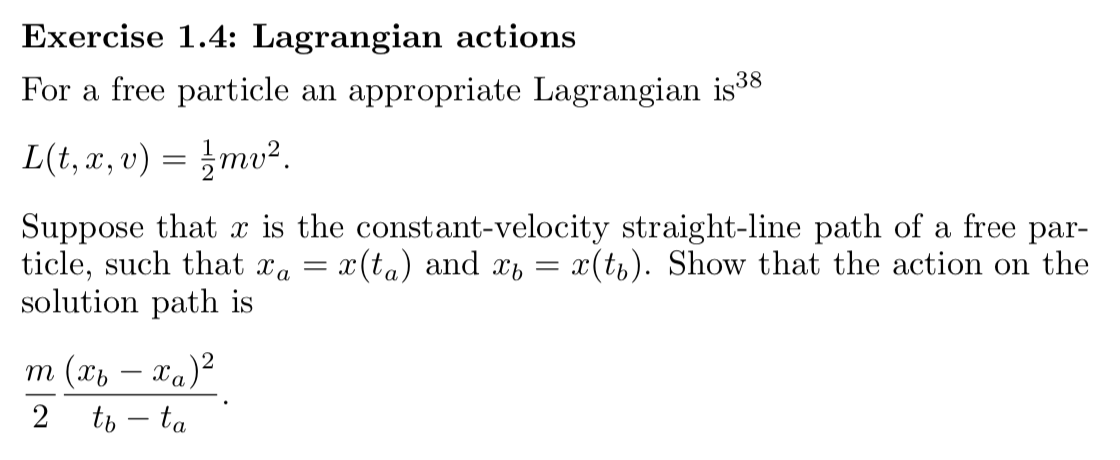
\includegraphics[width=400pt]{img/physics--classical-mechanics--sicm--1-4.png}
\end{mdframed}
The path function is
\begin{align*}
  x(t) = x_a + \frac{t - t_a}{t_b - t_a}(x_b - x_a).
\end{align*}
Therefore the velocity function is the constant function
\begin{align*}
  v(t) = (D x)(t) = \frac{x_b - x_a}{t_b - t_a}.
\end{align*}
Therefore the action is
\begin{align*}
  S[x](t_a, t_b) &= \int_{t_a}^{t_b}  \frac{1}{2}m \frac{(x_b - x_a)^2}{(t_b - t_a)^2} \d t \\
                 &= \frac{m}{2} \frac{(x_b - x_a)^2}{(t_b - t_a)^2}\int_{t_a}^{t_b} \d t \\
                 &= \frac{m}{2} \frac{(x_b - x_a)^2}{t_b - t_a}.
\end{align*}

% the dependence of the lagrangian on position is equal to the rate of change of the dependence of the lagrangian on velocity.